\section{Практическая часть}
\subsection{Разложение функции в ряд Фурье}{
  \textbf{Аналитически}

  Найдем разложение функции $f(x)=x^2$ в ряд Фурье на отрезке $[-\pi,\pi]$.
  
  Вычислим коэффициенты ряда Фурье:

  \begin{equation}
    a_0 = \frac{1}{\pi}\int_{-\pi}^{\pi} x^2 dx = \frac{1}{\pi}\left[\frac{x^3}{3}\right]_{-\pi}^{\pi} = \frac{1}{\pi}\left(\frac{\pi^3}{3} - \frac{-\pi^3}{3}\right) = \frac{2\pi^2}{3}
  \end{equation}


  \begin{equation}
    \begin{split}
    a_n & = \frac{1}{\pi}\int_{-\pi}^{\pi} x^2 \cos(nx) dx \\
    & = \frac{1}{\pi}\left[\frac{x^2\sin(nx)}{n} - \frac{2x\cos(nx)}{n^2} + \frac{2\sin(nx)}{n^3}\right]_{-\pi}^{\pi} \\
    & = \frac{1}{\pi}\left(\frac{\pi^2\sin(n\pi)}{n} - \frac{2\pi\cos(n\pi)}{n^2} + \frac{2\sin(n\pi)}{n^3} - \right. \\
    & \left. \frac{\pi^2\sin(-n\pi)}{n} + \frac{2\pi\cos(-n\pi)}{n^2} - \frac{2\sin(-n\pi)}{n^3}\right) \\
    & = \frac{4}{n^2}(-1)^n, \quad n \geq 1
    \end{split}
  \end{equation}

  \begin{equation}
    \begin{split}
    b_n & = \frac{1}{\pi}\int_{-\pi}^{\pi} x^2 \sin(nx) dx \\
    & = \frac{1}{\pi}\left[-\frac{x^2\cos(nx)}{n} + \frac{2x\sin(nx)}{n^2} + \frac{2\cos(nx)}{n^3}\right]_{-\pi}^{\pi} \\
    & = 0, \quad n \geq 1
    \end{split}
  \end{equation}

  Таким образом, ряд Фурье для функции $f(x)=x^2$ имеет вид:

  \begin{equation}
    f(x) = \frac{\pi^2}{3} + 4\sum_{n=1}^{\infty} \frac{(-1)^n}{n^2}\cos(nx)
  \end{equation}

  \textbf{в Maple}
    \begin{lstlisting}[style=maple]
      f:=x^2
      plot(f)
    \end{lstlisting}
    Для подтверждения правильности решения, можно построить график функции $f(x)=x^2$.
   
      \begin{center}
        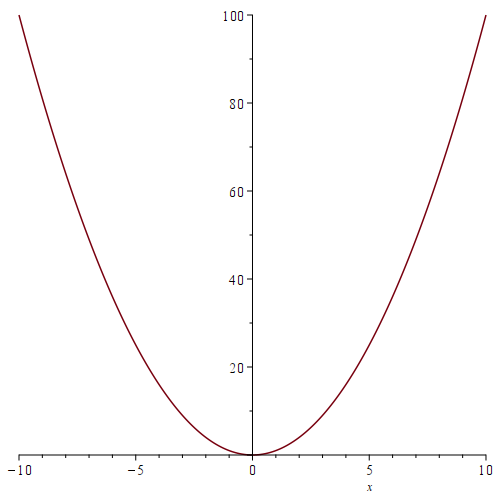
\includegraphics[width=0.7\textwidth]{2.png}  % Adjust filename and width as needed
        \end{center}
        \begin{lstlisting}[style=maple]
      l := 1/Pi
     a0:=l*int(f,x=-Pi..Pi)
     an:=l*int(f*cos(n*x),x=-Pi..Pi)
     bn:=l*int(f*sin(n*x),x=-Pi..Pi)
     s:=a0/2+sum(an*cos(n*x)+bn*sin(n*x),n=1..100)
     plot([f,s],x=-Pi..Pi)
        \end{lstlisting}
        
        \begin{center}
        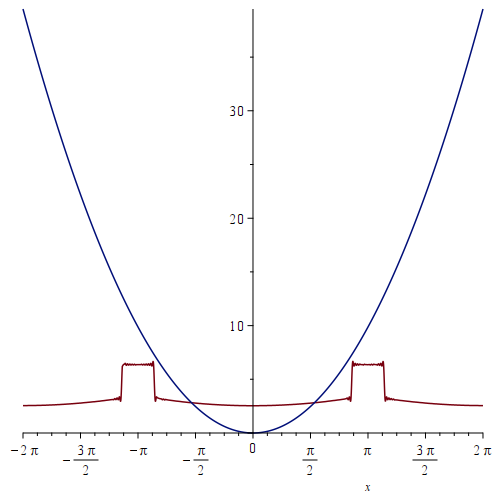
\includegraphics[width=0.7\textwidth]{1.png}  % Adjust filename and width as needed
        \end{center}
Мы видим, что разложение в ряд Фурье функции $f(x)=x^2$ сходится к функции $f(x)=x^2$ на
промежутке $[-\pi,\pi]$.
        }

\subsection{Косинус преобразование функции}{
  \textbf{Аналитически}


  Найдем косинус-преобразование Фурье для функции:
  \[
  f(x) = \begin{cases}
  1, & |x| \leq l \\
  0, & l < |x|
  \end{cases}
  \]
  
  Косинус-преобразование Фурье с нормировочным множителем определяется как:
  \[
  F_c(\omega) = \sqrt{\frac{2}{\pi}} \int_{-\infty}^{\infty} f(x) \cos(\omega x) \, dx
  \]
  
  Учитывая четность функции и области определения:
  \begin{equation}
  \begin{split}
  F_c(\omega) &= \sqrt{\frac{2}{\pi}} \int_{-l}^{l} 1 \cdot \cos(\omega x) \, dx \\
  &= \sqrt{\frac{2}{\pi}} \cdot 2\int_{0}^{l} \cos(\omega x) \, dx \\
  &= \sqrt{\frac{2}{\pi}} \cdot 2 \left[\frac{\sin(\omega x)}{\omega}\right]_{0}^{l} \\
  &= \sqrt{\frac{2}{\pi}} \cdot 2 \left(\frac{\sin(\omega l)}{\omega}\right) \\
  &= \sqrt{\frac{2}{\pi}} \cdot \frac{2\sin(\omega l)}{\omega} \\
  &= \sqrt{\frac{2}{\pi}} \sin(\omega l)
  \end{split}
  \end{equation}
  
  Таким образом, косинус-преобразование Фурье заданной функции имеет вид:
  \[
  F_c(\omega) = \sqrt{\frac{2}{\pi}} \sin(\omega l)
  \]
  }

  \textbf{в Maple}
  Рассмотрим задачу нахождения косинус преобразование заданной функции
  \begin{center}Пример задачи 1
    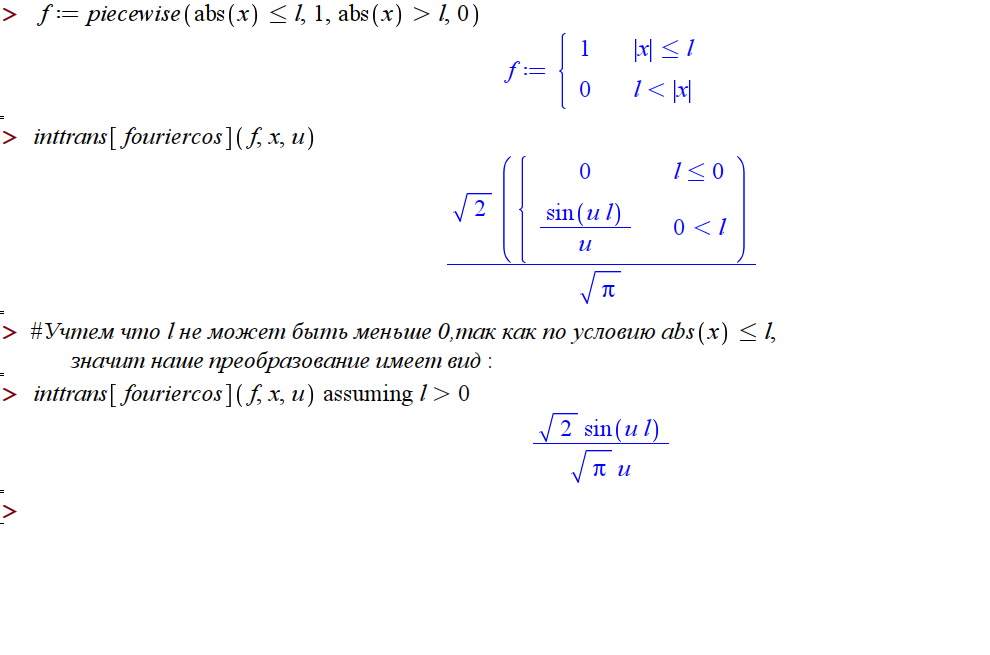
\includegraphics[width=0.7\textwidth]{practice_2.png}  
    \end{center}
   
}



\subsection{Нахождение изображение от функции оригинала}{
  \textbf{Аналитически}

  Найдем изображение по Лапласу для функции:
  \[
  f(t) = \begin{cases}
  0, & t \leq 0 \\
  1 - \frac{t}{a}, & 0 < t \leq 2a \\
  -3 + \frac{t}{a}, & 2a < t \leq 3a \\
  0, & t > 3a
  \end{cases}
  \]
  
  Разобьем интеграл на части:
  \begin{equation}
  \begin{split}
  L\{f(t)\} &= \int_{0}^{2a} (1 - \frac{t}{a})e^{-pt}dt + \int_{2a}^{3a} (-3 + \frac{t}{a})e^{-pt}dt \\
  &= \frac{1}{p} - \frac{1}{ap}\int_{0}^{2a} te^{-pt}dt - 3\int_{2a}^{3a} e^{-pt}dt + \frac{1}{a}\int_{2a}^{3a} te^{-pt}dt
  \end{split}
  \end{equation}
  
  После интегрирования получаем:
  \begin{equation}
  \begin{split}
  L\{f(t)\} &= \frac{1}{p} - \frac{1}{p^2}(1 + e^{-3p} - 2e^{-2p}) \\
  \end{split}
  \end{equation}
  
  Таким образом, изображение по Лапласу имеет вид:
  \[
  F(p) = \frac{1}{p} - \frac{1 + e^{-3p} - 2e^{-2p}}{p^2}
  \]


  \textbf{в Maple}
  По данному графику функции-оригинала найти ее изображе-
  ние Лапласа.
  \begin{center}
    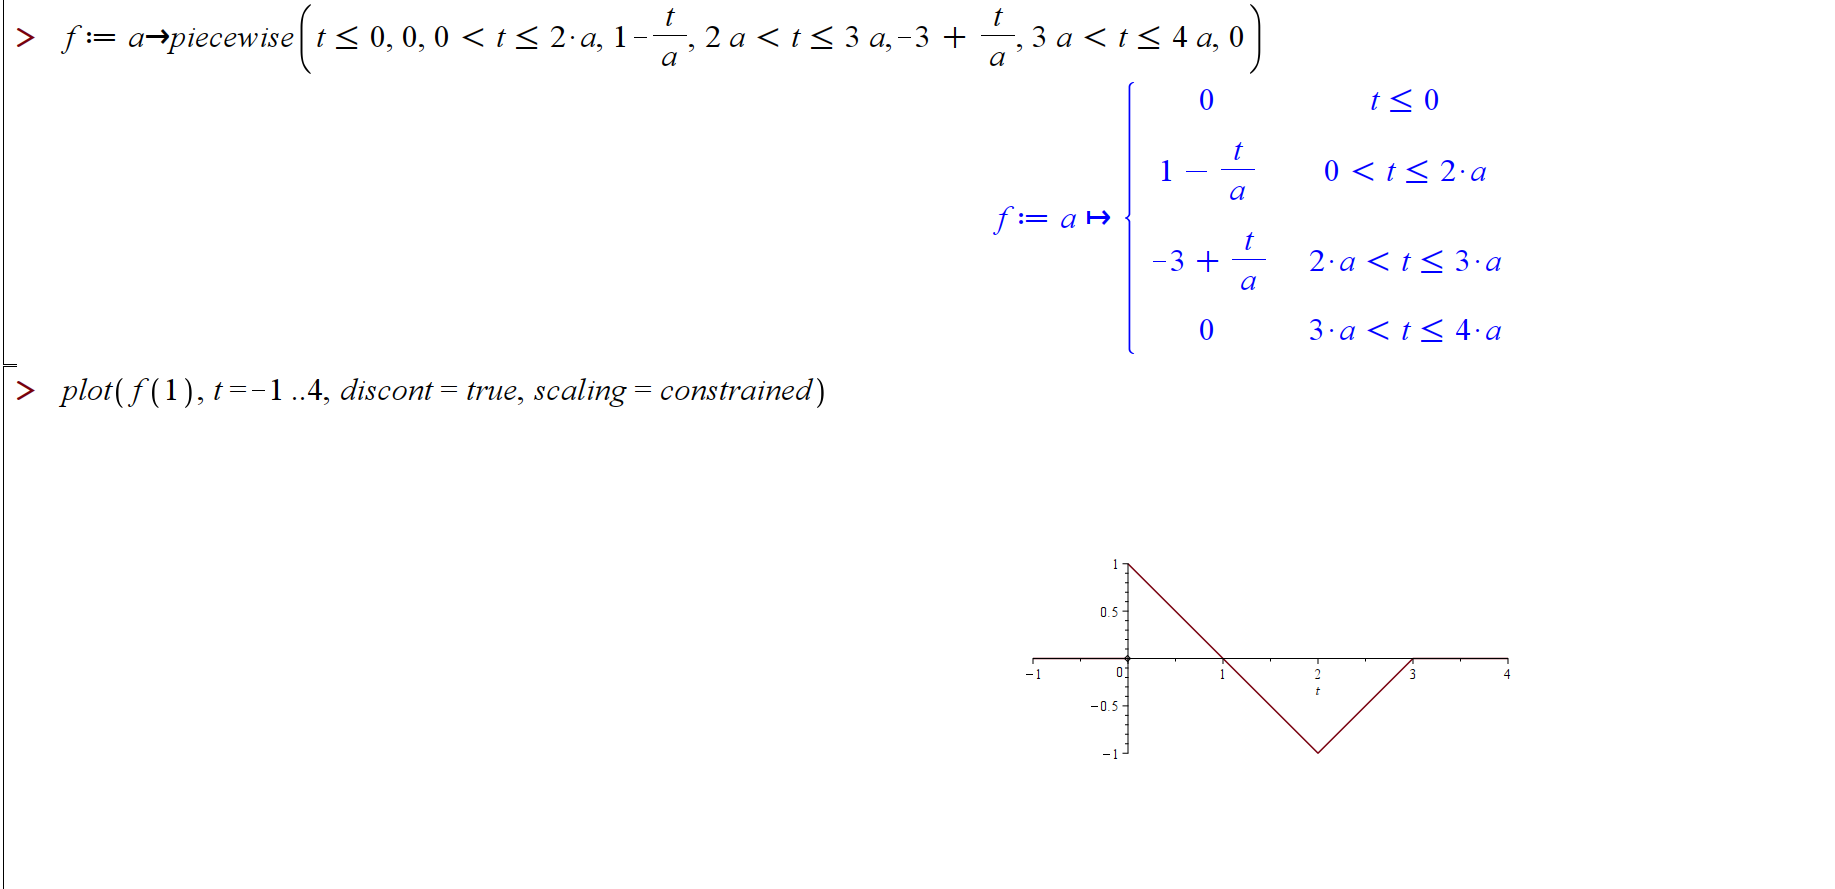
\includegraphics[width=1.0\textwidth]{practice(4_1).png} 
    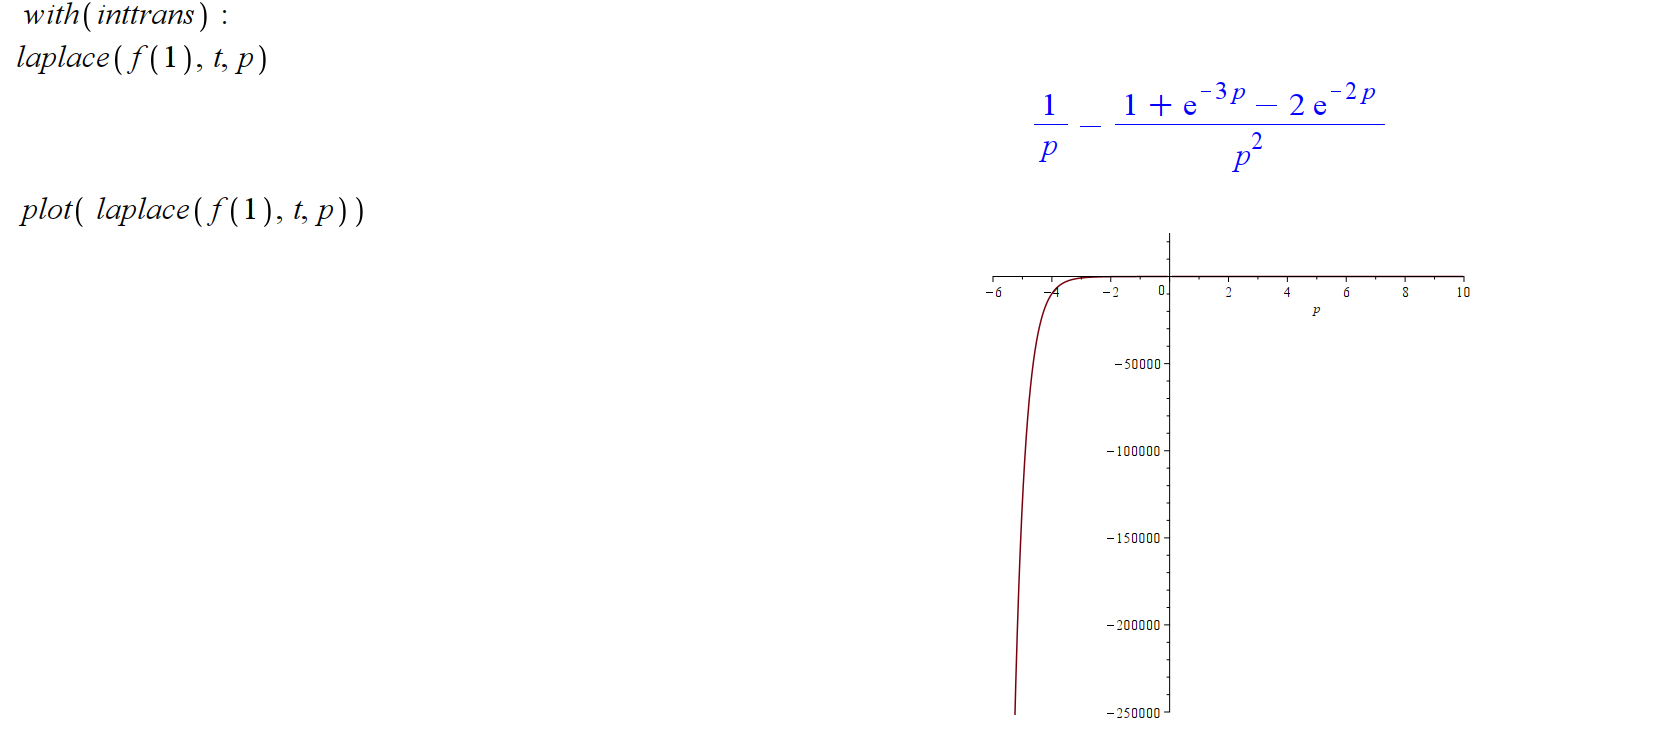
\includegraphics[width=1.0\textwidth]{practice(4_2).png} 
    \end{center}
}
\subsection{Интеграл Фурье}{
  \textbf{Аналитически}
  Найдем интеграл Фурье для функции $f(x) = e^{-\alpha|x|}\sin(\beta x)$:

  \begin{equation}
  \begin{split}
  F(\omega) &= \int_{-\infty}^{\infty} e^{-\alpha|x|}\sin(\beta x)e^{-i\omega x}dx \\
  &= \int_{-\infty}^{0} e^{\alpha x}\sin(\beta x)e^{-i\omega x}dx + 
     \int_{0}^{\infty} e^{-\alpha x}\sin(\beta x)e^{-i\omega x}dx
  \end{split}
  \end{equation}
  
  Для первого интеграла:
  \begin{equation}
  \begin{split}
  I_1 &= \int_{-\infty}^{0} e^{\alpha x}\sin(\beta x)e^{-i\omega x}dx \\
  &= \int_{-\infty}^{0} e^{(\alpha-i\omega)x}\sin(\beta x)dx \\
  &= \frac{\beta}{(\alpha-i\omega)^2 + \beta^2}
  \end{split}
  \end{equation}
  Для второго интеграла:
  \begin{equation}
  \begin{split}
  I_2 &= \int_{0}^{\infty} e^{-\alpha x}\sin(\beta x)e^{-i\omega x}dx \\
  &= \int_{0}^{\infty} e^{-(\alpha+i\omega)x}\sin(\beta x)dx \\
  &= \frac{\beta}{(\alpha+i\omega)^2 + \beta^2}
  \end{split}
  \end{equation}
  
  Суммируя $I_1$ и $I_2$:
  \begin{equation}
  \begin{split}
  F(\omega) &= I_1 + I_2 \\
  &= \frac{\beta}{(\alpha-i\omega)^2 + \beta^2} + \frac{\beta}{(\alpha+i\omega)^2 + \beta^2} \\
  &= \frac{2\alpha\beta}{(\alpha^2+\omega^2-\beta^2)^2 + 4\alpha^2\beta^2}
  \end{split}
  \end{equation}
  
  Таким образом, интеграл Фурье равен:
  \[
  F(\omega) = \frac{2\alpha\beta}{(\alpha^2+\omega^2-\beta^2)^2 + 4\alpha^2\beta^2}
  \]
  }


  \textbf{в Maple}
  Рассмотрим задачу представление функции интегралом фурье 
  \begin{center}
    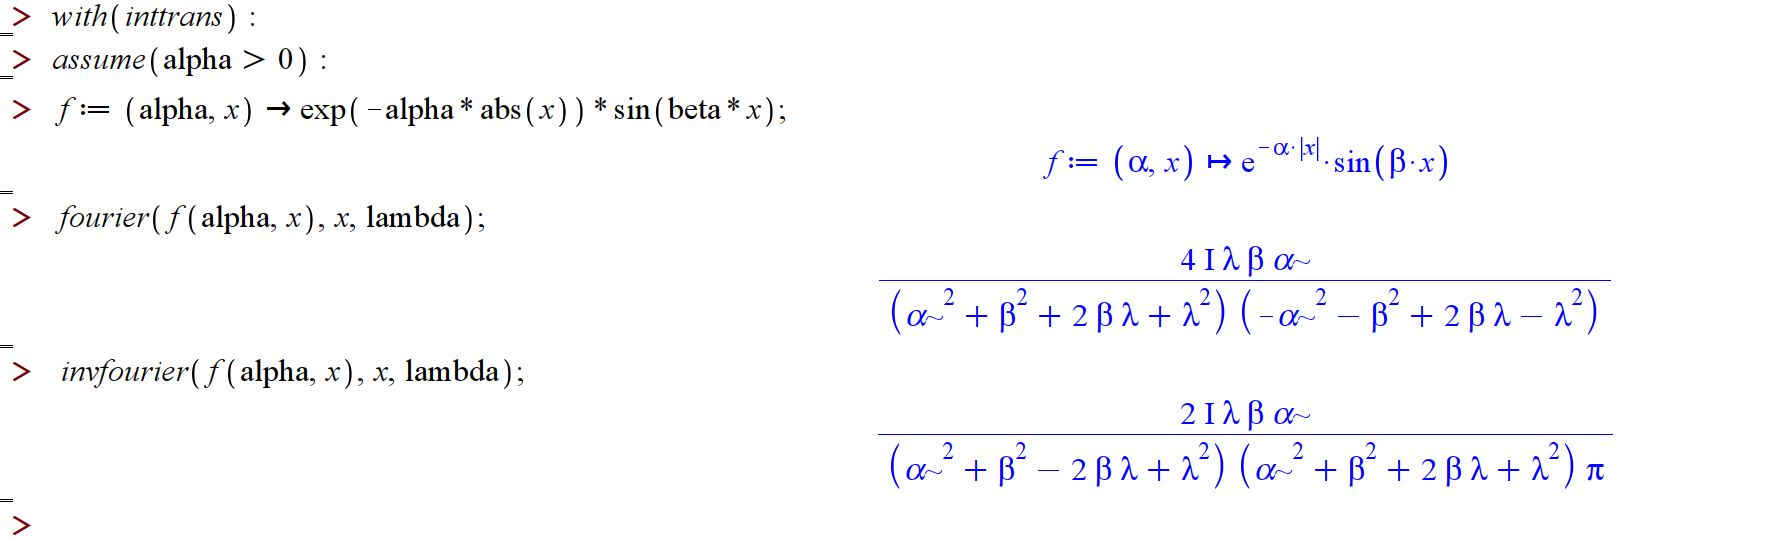
\includegraphics[width=1.0\textwidth]{practice_5.png}  
    \end{center}
}
\subsection{Преобразование сигналов}{
  \textbf{Аналитически}




  \textbf{в Maple}
  Протестируем работу различных функций преобразования Фурье системы
компьютерного анализа Maple на сигнале $sin(t)$*\exp(-t^2/200)$
 

\begin{center}{
  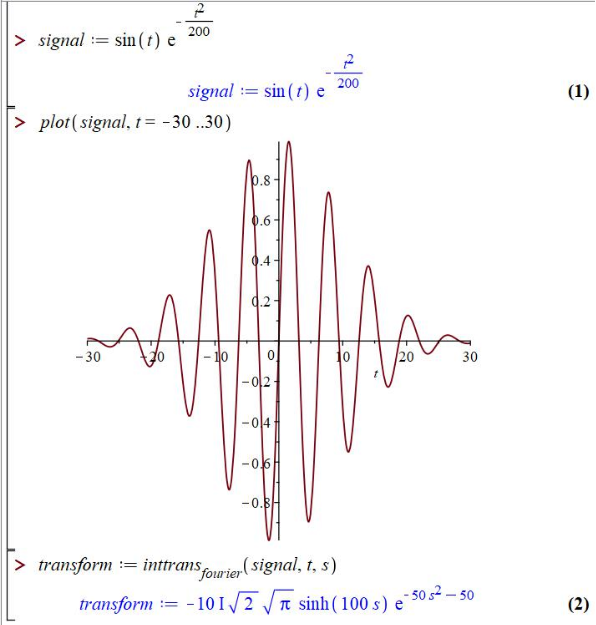
\includegraphics[width=0.7\textwidth]{signal1.png} 
  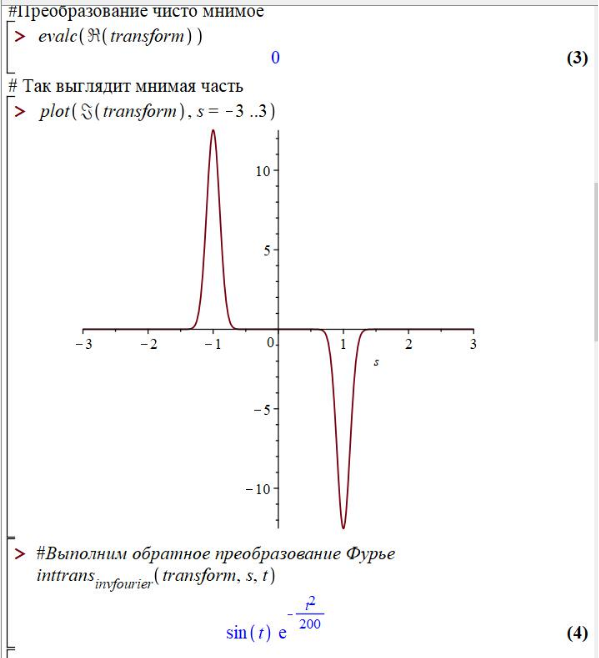
\includegraphics[width=0.7\textwidth]{signal2.png} 
  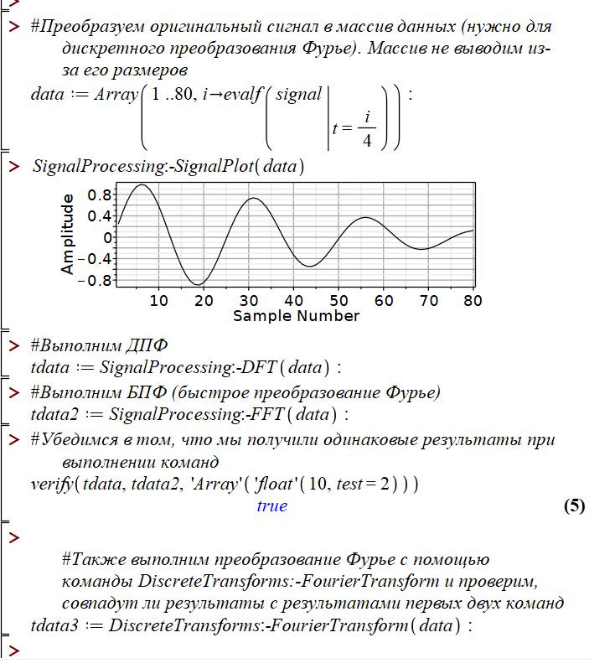
\includegraphics[width=0.7\textwidth]{signal3.png} 
  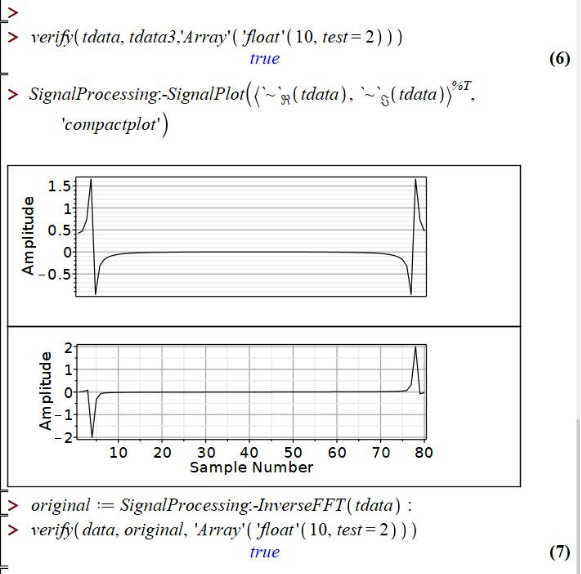
\includegraphics[width=0.7\textwidth]{signal4.png} 

  \end{center}

}


\subsection {Аппроксимация изображения}{
  Рассмотрим алгоритм сжатия картинки при помощи рядов Фурье. Алгоритм сжатия изображения
   с использованием рядов Фурье основан на представлении изображения в частотной области.
    В этом представлении низкочастотные компоненты описывают основную структуру изображения,
     а высокочастотные — мелкие детали. Процесс сжатия заключается в удалении высокочастотных компонентов,
      которые вносят минимальный вклад в визуальное восприятие, и последующем восстановлении изображения.
      Для изображения $I(x, y)$, заданного на дискретной решётке размером $N \times M$, дискретное двумерное преобразование Фурье задаётся формулой:
\[
F(u, v) = \sum_{x=0}^{N-1} \sum_{y=0}^{M-1} I(x, y) e^{-j 2 \pi \left( \frac{ux}{N} + \frac{vy}{M} \right)},
\]
где:
\begin{itemize}
    \item $F(u, v)$ — коэффициенты преобразования Фурье (комплексные числа),
    \item $u, v$ — пространственные частоты,
    \item $j$ — мнимая единица ($j^2 = -1$).
\end{itemize}

Обратное преобразование Фурье:
\[
I(x, y) = \frac{1}{NM} \sum_{u=0}^{N-1} \sum_{v=0}^{M-1} F(u, v) e^{j 2 \pi \left( \frac{ux}{N} + \frac{vy}{M} \right)}.
\]
}


\textbf{Сжатие изображения}{

Процесс сжатия выполняется следующим образом:
\begin{enumerate}
    \item Выполняем дискретное преобразование Фурье (ДПФ) для исходного изображения $I(x, y)$, получая $F(u, v)$.
    \item Устанавливаем в нуль коэффициенты $F(u, v)$, абсолютные значения которых меньше некоторого порога $T$:
    \[
    F'(u, v) = 
    \begin{cases} 
    F(u, v), & \text{если } |F(u, v)| \geq T, \\
    0, & \text{если } |F(u, v)| < T.
    \end{cases}
    \]
    \newpage
    \item Выполняем обратное преобразование Фурье с $F'(u, v)$, получая сжатое изображение $I'(x, y)$.
\end{enumerate}
  
Рассмотрим пример сжатия картинки 

\begin{figure}[h!]
  \centering
  % Первая картинка
  \begin{subfigure}[b]{0.45\textwidth}
      \centering
      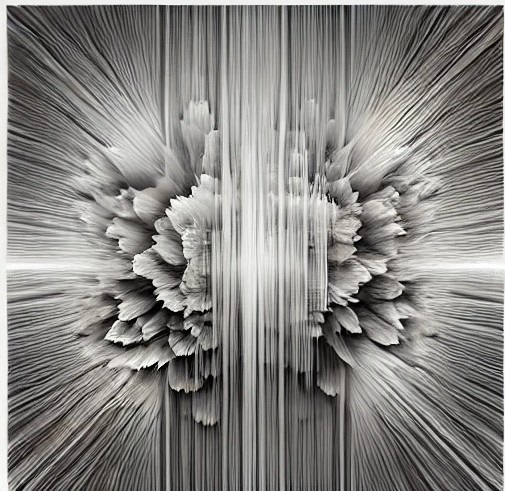
\includegraphics[width=\textwidth]{FourierBefore.jpeg} % Путь к первой картинке
      \caption{Оригинальное изображение}
      \label{fig:original}
  \end{subfigure}
  \hfill
  % Вторая картинка
  \begin{subfigure}[b]{0.45\textwidth}
      \centering
      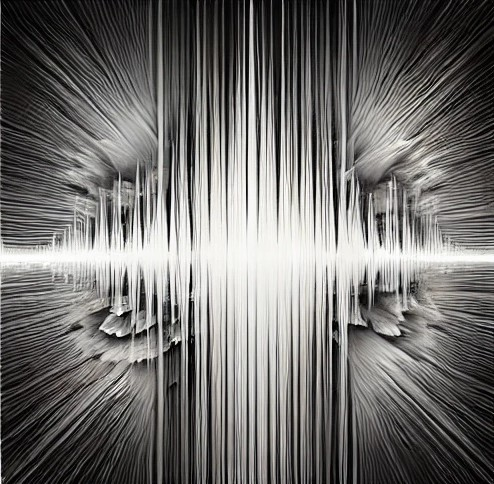
\includegraphics[width=\textwidth]{FourierAfter.jpeg} % Путь ко второй картинке
      \caption{Сжатое изображение}
      \label{fig:compressed}
  \end{subfigure}
  \caption{Сравнение оригинального и сжатого изображения.}
  \label{fig:comparison}
\end{figure}

}

